\documentclass[11pt]{article}
\usepackage[margin=0.72in]{geometry}
\usepackage{graphicx}
\usepackage{booktabs}
\usepackage{caption}
\usepackage{enumitem}
\usepackage{float}
\setlength{\parindent}{0pt}
\setlength{\parskip}{4pt}
\captionsetup{font=small}
\begin{document}

\begin{center}
    {\Large \textbf{Proposal: Smart-City Traffic Analysis using NYC Taxi Trips}}\\[6pt]
    {\normalsize CS F415 Data Mining \quad|\quad Group 5}\\[3pt]
    {\small
    Chaitanya Keyal (2023B4A70727H) \quad
    Alex Antony (2023B4A70734H)\\
    Abhishek Verma (2023B4A71256H) \quad
    Tanmay Goel (2023A7PS0027H)
    }
\end{center}

\textbf{1. Executive Summary}\
A Municipal Corporation requires data-driven interventions to reduce traffic congestion and improve transit planning. We analyzed the NYC Taxi Trip Duration dataset with \textbf{1,458,644} trips from \textbf{January 1, 2016 to June 30, 2016}. The dataset contains 11 features including pickup/dropoff timestamps, GPS coordinates, passenger count, and trip duration. This proposal defines three linked data mining tasks: (1) \textit{trip duration prediction} for travel-time estimation and anomaly detection, (2) \textit{spatial demand clustering} for high-demand zone discovery, and (3) \textit{congestion-level classification} for dynamic transit scheduling and traffic response.

\textbf{2. Data Exploration Summary}\
The dataset is complete (no missing values) and temporally consistent (no pickup-after-dropoff records; no mismatch between computed and provided duration). Basic profiling indicates heavy right-skew in trip duration and strong time-of-day effects in both trip counts and speed.

\textbf{Key Statistics}
\begin{table}[H]
    \centering
    \small
    \begin{tabular}{@{}ll@{}}
        \toprule
        Metric                                 & Value                    \\
        \midrule
        Total records                          & 1,458,644                \\
        Features                               & 11                       \\
        Date range                             & 2016-01-01 to 2016-06-30 \\
        Mean / median trip duration            & 959.49 s / 662 s         \\
        Trip duration standard deviation       & 5,237.43 s               \\
        Mean / median Haversine distance       & 3.441 km / 2.094 km      \\
        Median estimated speed (overall)       & 12.792 km/h              \\
        Median speed: peak vs off-peak         & 11.851 vs 19.180 km/h    \\
        Trips during peak hours (7--9, 17--19) & 30.69\%                  \\
        Vendor split (1 / 2)                   & 46.50\% / 53.50\%        \\
        \bottomrule
    \end{tabular}
\end{table}

\textbf{Data Quality Findings}
\begin{itemize}[leftmargin=1.4em,itemsep=2pt,topsep=2pt]
    \item Coordinates outside NYC bounds (40.4--41.0 N, -74.3 to -73.7 W): \textbf{985 trips} (0.0675\%); invalid pickups: 247, invalid dropoffs: 971.
    \item Short-duration anomalies ($<$60 s): \textbf{8,595 trips} (0.5892\%); long-duration anomalies ($>$24 h): \textbf{4 trips}.
    \item Passenger-count anomalies: \textbf{60} zero-passenger trips; \textbf{5} trips with $>$6 passengers.
    \item Estimated speed anomalies ($>$100 km/h): \textbf{175 trips}; zero-distance trips: \textbf{5,897}.
\end{itemize}

\textbf{Notable Patterns}
\begin{itemize}[leftmargin=1.4em,itemsep=2pt,topsep=2pt]
    \item Demand shows clear commute peaks in morning and evening hours.
    \item Median speed drops during peak windows, indicating higher congestion.
    \item Spatial demand is concentrated around core Manhattan and major airport corridors.
\end{itemize}

\begin{figure}[H]
    \centering
    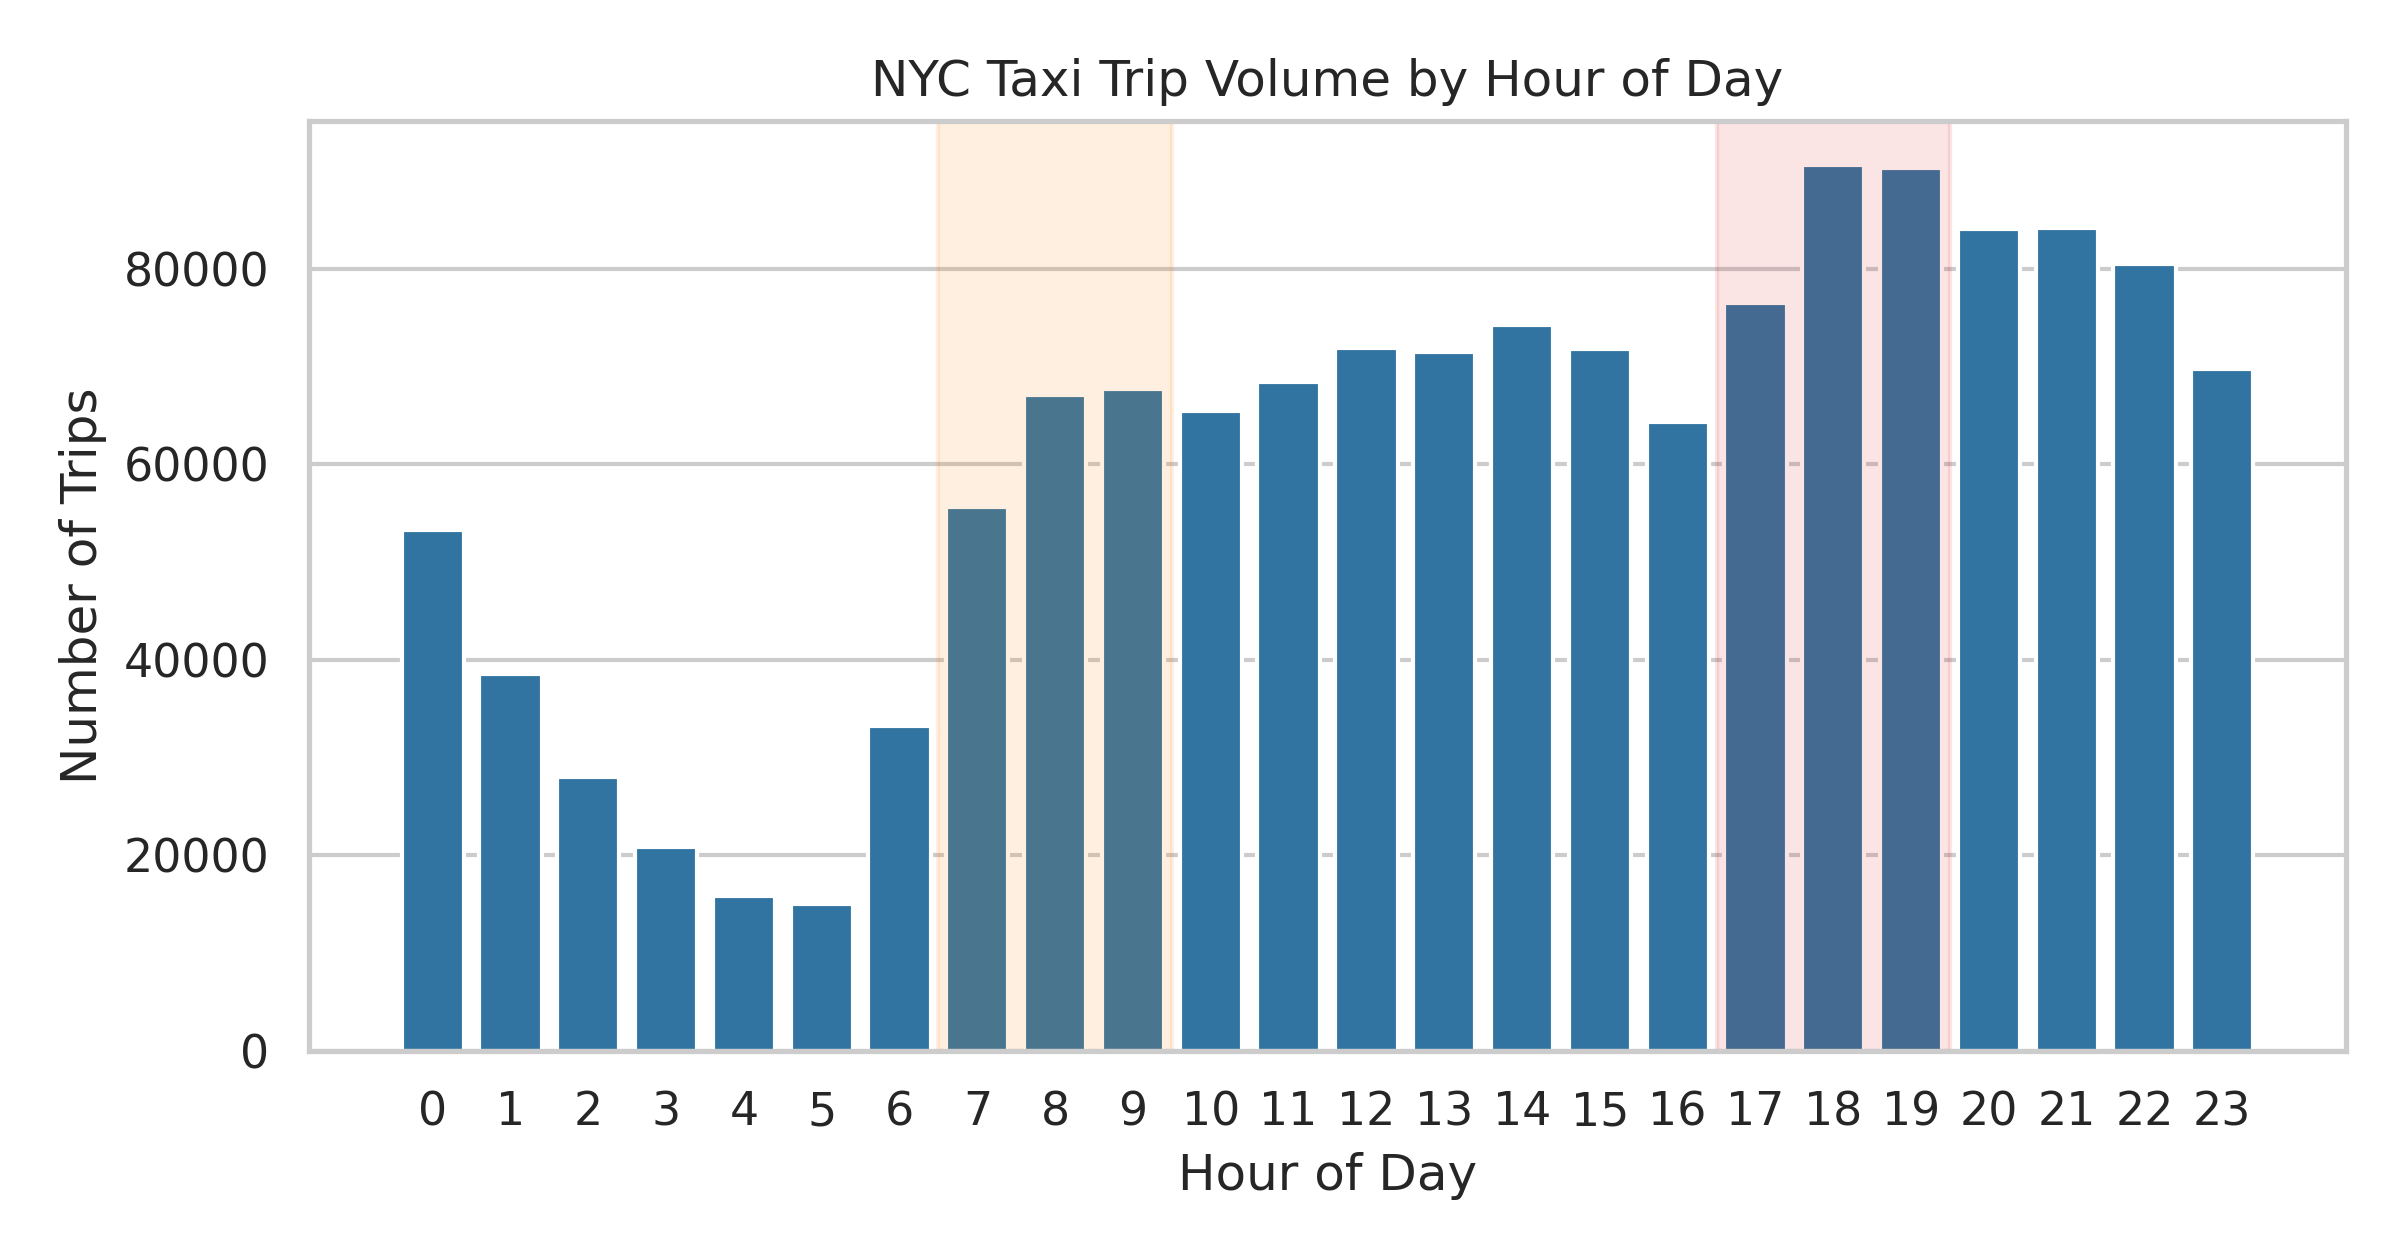
\includegraphics[width=0.48\textwidth]{../figures/trip_volume_by_hour.png}\hfill
    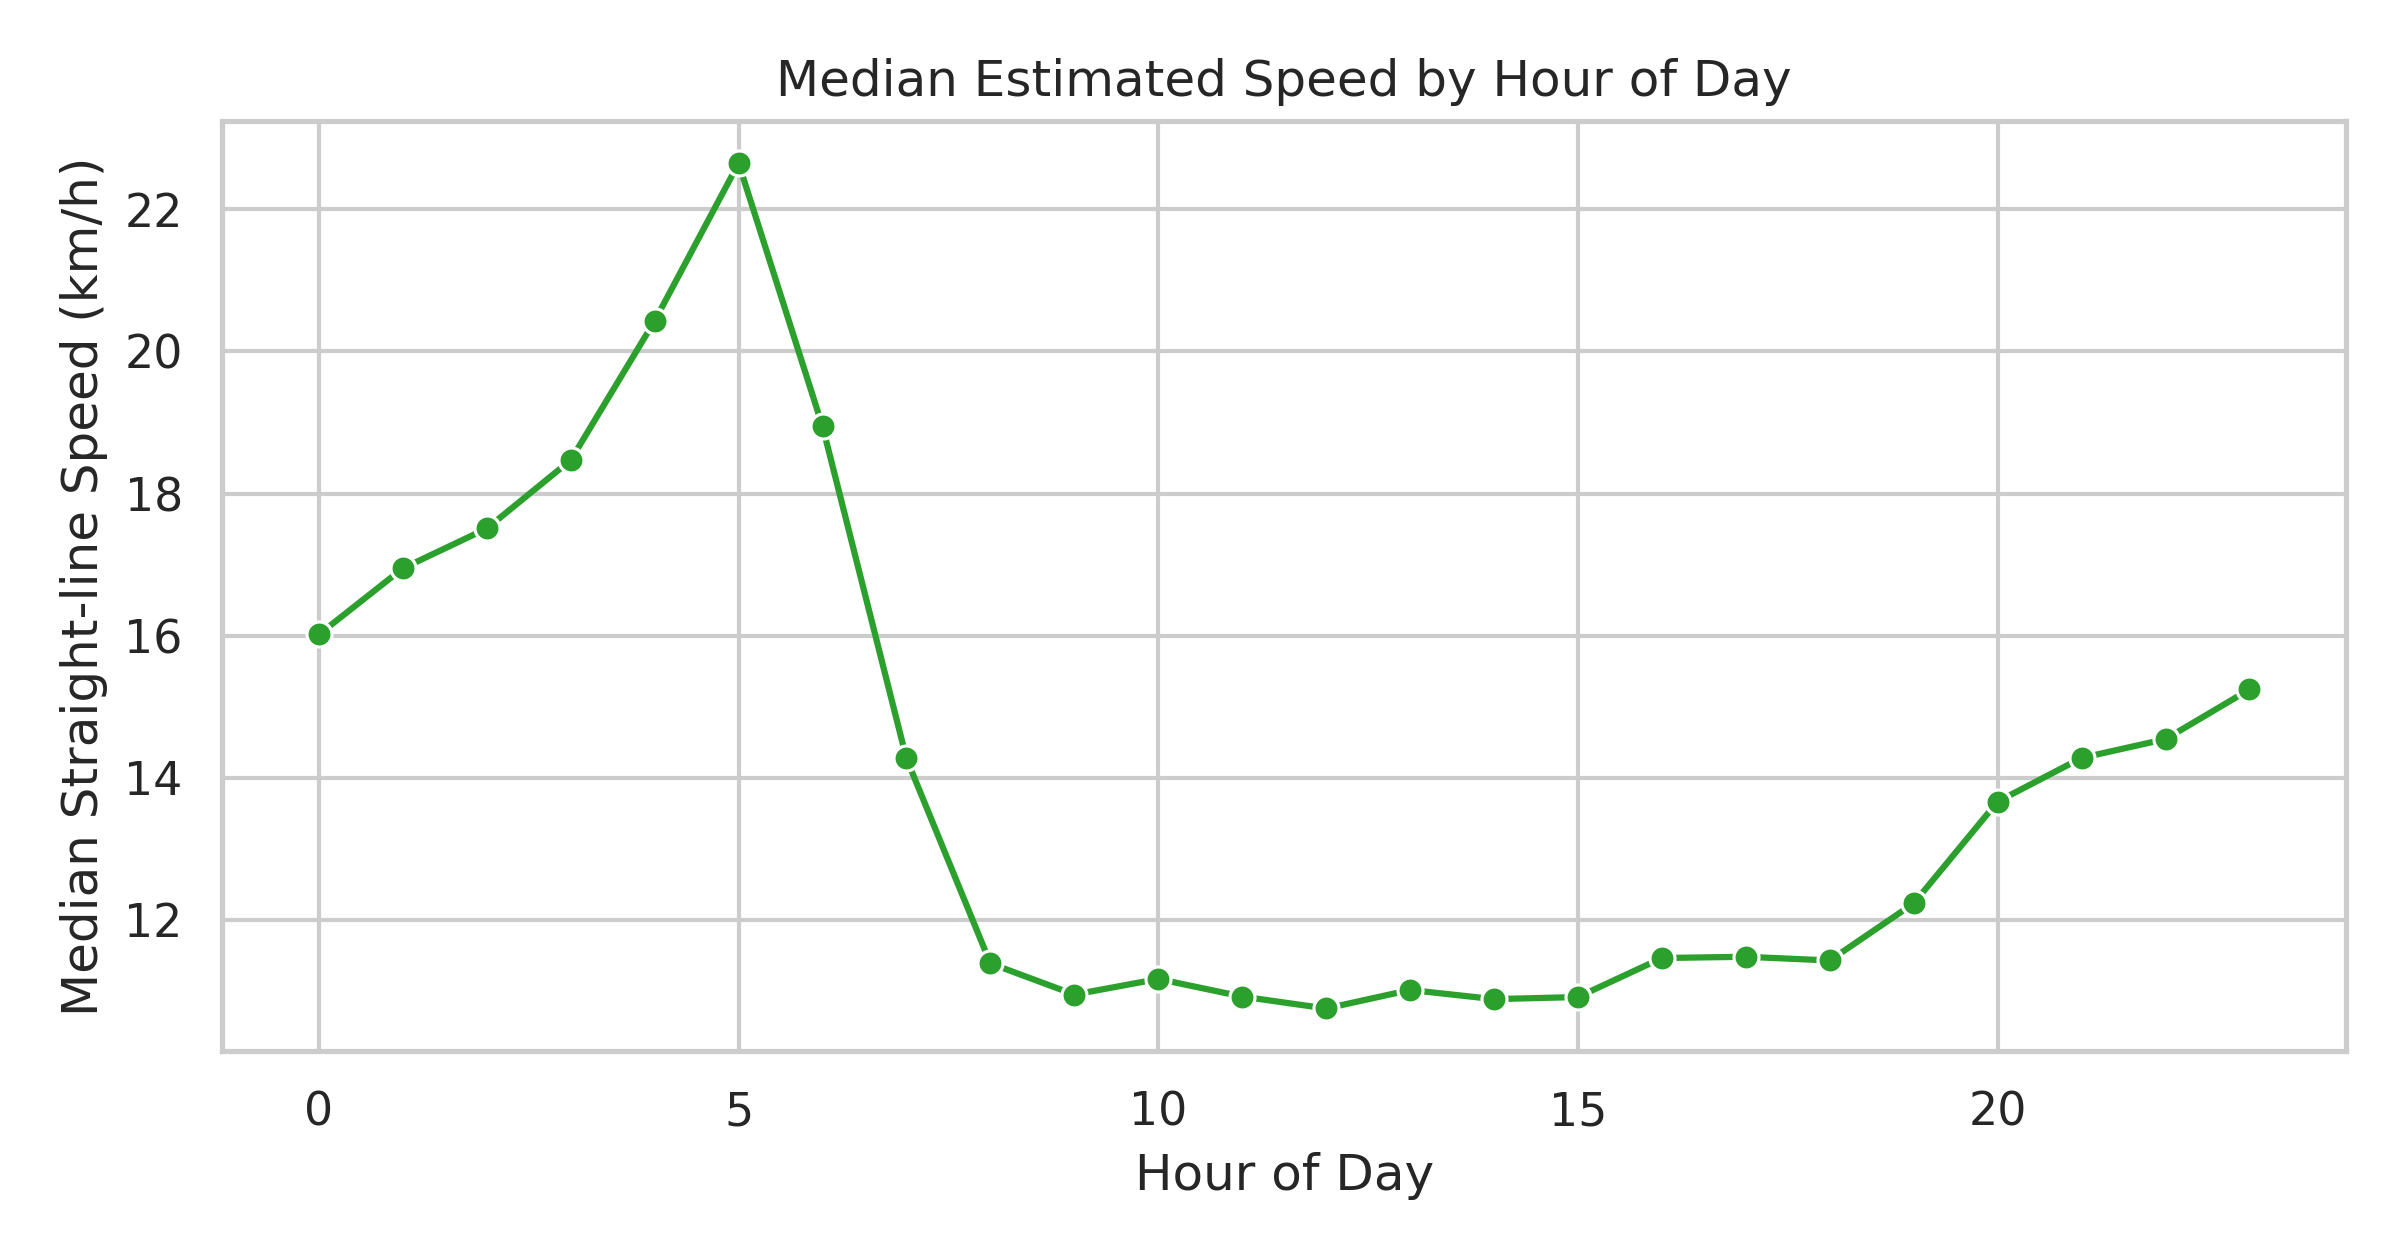
\includegraphics[width=0.48\textwidth]{../figures/speed_by_hour.png}
    \caption{Left: hourly trip demand reveals AM/PM peak periods. Right: median straight-line speed dips during rush hours, a direct congestion proxy.}
\end{figure}

\textbf{3. Problem Formulation}

\textbf{Task 1: Trip Duration Prediction (Supervised Regression)}\\
\textit{Input $\rightarrow$ Output:} Temporal features (hour, weekday, month), pickup/dropoff coordinates, vendor/passenger fields, Haversine distance $\rightarrow$ predicted trip duration (seconds).
\begin{itemize}[leftmargin=1.2em,itemsep=1pt,topsep=2pt]
    \item[\textbullet] Travel-time forecasting for route planning and passenger information systems
    \item[\textbullet] Real-time incident flagging when actual duration greatly exceeds prediction
    \item[\textbullet] Dynamic bus/subway capacity allocation on parallel corridors
    \item[\textbullet] Evidence base for time-zone congestion pricing
\end{itemize}
\textit{Planned models:} Linear Regression, Random Forest, Gradient Boosting.

\vspace{0.5em}
\textbf{Task 2: High-Demand Zone Identification (Unsupervised Clustering)}\\
\textit{Input $\rightarrow$ Output:} Pickup coordinates (optionally enriched with demand counts and mean duration) $\rightarrow$ cluster labels representing geographic demand zones.
\begin{itemize}[leftmargin=1.2em,itemsep=1pt,topsep=2pt]
    \item[\textbullet] Identify underserved high-demand areas for transit augmentation
    \item[\textbullet] Prioritize zones for traffic signal and lane interventions
    \item[\textbullet] Guide park-and-ride or bike-share station placement
    \item[\textbullet] Inform zone-based congestion pricing and infrastructure spending
\end{itemize}
\textit{Planned models:} K-Means \textbf{vs.}\ DBSCAN (algorithm comparison).

\vspace{0.5em}
\textbf{Task 3: Congestion Level Classification (Supervised Multi-class)}\\
\textit{Input $\rightarrow$ Output:} Zone ID, hour, weekday, historical trip count, and average speed $\rightarrow$ congestion class \{High, Medium, Low\}. Labels derived via speed-percentile thresholds across zone--time buckets.
\begin{itemize}[leftmargin=1.2em,itemsep=1pt,topsep=2pt]
    \item[\textbullet] Dynamic public-transit service frequency control
    \item[\textbullet] Commuter-facing congestion alerts and route suggestions
    \item[\textbullet] Optimized staffing and operations planning for transit agencies
    \item[\textbullet] Data-backed policy support for staggered work hours
\end{itemize}
\textit{Planned models:} Logistic Regression, Random Forest Classifier.

\textbf{4. Expected Outcomes \& Next Steps}\
Phase 2 (Weeks 9--15) will operationalize these tasks through preprocessing, feature pipeline finalization, weather-data integration, model comparison, and failure analysis. Expected outcomes are actionable recommendations such as targeted peak-hour bus deployment, high-friction zone interventions, and evidence-based congestion pricing policies linked to measured speed and demand patterns.

\end{document}
